% Created by tikzDevice version 0.12.6 on 2025-07-14 15:46:04
% !TEX encoding = UTF-8 Unicode
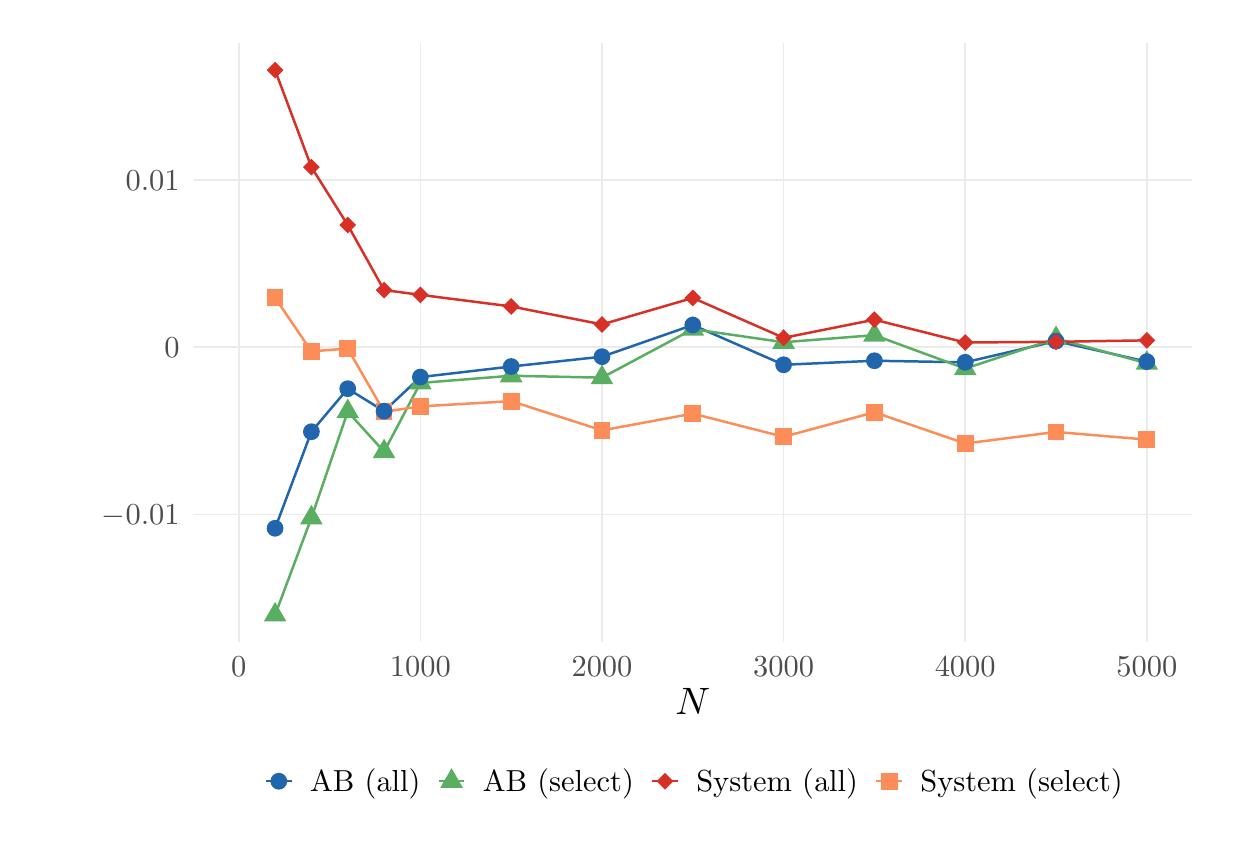
\begin{tikzpicture}[x=1pt,y=1pt]
\definecolor{fillColor}{RGB}{255,255,255}
\path[use as bounding box,fill=fillColor,fill opacity=0.00] (0,0) rectangle (433.62,289.08);
\begin{scope}
\path[clip] ( 59.87, 67.02) rectangle (420.81,283.58);
\definecolor{drawColor}{gray}{0.92}

\path[draw=drawColor,line width= 0.6pt,line join=round] ( 59.87,113.21) --
	(420.81,113.21);

\path[draw=drawColor,line width= 0.6pt,line join=round] ( 59.87,173.68) --
	(420.81,173.68);

\path[draw=drawColor,line width= 0.6pt,line join=round] ( 59.87,234.15) --
	(420.81,234.15);

\path[draw=drawColor,line width= 0.6pt,line join=round] ( 76.28, 67.02) --
	( 76.28,283.58);

\path[draw=drawColor,line width= 0.6pt,line join=round] (141.90, 67.02) --
	(141.90,283.58);

\path[draw=drawColor,line width= 0.6pt,line join=round] (207.53, 67.02) --
	(207.53,283.58);

\path[draw=drawColor,line width= 0.6pt,line join=round] (273.15, 67.02) --
	(273.15,283.58);

\path[draw=drawColor,line width= 0.6pt,line join=round] (338.78, 67.02) --
	(338.78,283.58);

\path[draw=drawColor,line width= 0.6pt,line join=round] (404.40, 67.02) --
	(404.40,283.58);
\definecolor{drawColor}{RGB}{33,102,172}

\path[draw=drawColor,line width= 0.9pt,line join=round] ( 89.40,108.18) --
	(102.53,143.08) --
	(115.65,158.62) --
	(128.78,150.50) --
	(141.90,162.82) --
	(174.72,166.64) --
	(207.53,170.19) --
	(240.34,181.63) --
	(273.15,167.27) --
	(305.97,168.72) --
	(338.78,168.16) --
	(371.59,175.81) --
	(404.40,168.40);
\definecolor{drawColor}{RGB}{90,174,97}

\path[draw=drawColor,line width= 0.9pt,line join=round] ( 89.40, 76.86) --
	(102.53,111.96) --
	(115.65,150.34) --
	(128.78,135.87) --
	(141.90,160.70) --
	(174.72,163.30) --
	(207.53,162.61) --
	(240.34,180.14) --
	(273.15,175.41) --
	(305.97,177.97) --
	(338.78,165.89) --
	(371.59,176.75) --
	(404.40,167.82);
\definecolor{drawColor}{RGB}{215,48,39}

\path[draw=drawColor,line width= 0.9pt,line join=round] ( 89.40,273.74) --
	(102.53,238.69) --
	(115.65,217.76) --
	(128.78,194.26) --
	(141.90,192.53) --
	(174.72,188.35) --
	(207.53,181.84) --
	(240.34,191.42) --
	(273.15,177.01) --
	(305.97,183.56) --
	(338.78,175.31) --
	(371.59,175.57) --
	(404.40,176.09);
\definecolor{drawColor}{RGB}{252,141,89}

\path[draw=drawColor,line width= 0.9pt,line join=round] ( 89.40,191.49) --
	(102.53,172.12) --
	(115.65,173.13) --
	(128.78,150.29) --
	(141.90,152.23) --
	(174.72,154.13) --
	(207.53,143.56) --
	(240.34,149.62) --
	(273.15,141.24) --
	(305.97,150.11) --
	(338.78,138.82) --
	(371.59,142.99) --
	(404.40,140.23);
\definecolor{fillColor}{RGB}{90,174,97}

\path[fill=fillColor] (141.90,165.42) --
	(145.99,158.35) --
	(137.82,158.35) --
	cycle;
\definecolor{fillColor}{RGB}{252,141,89}

\path[fill=fillColor] (138.87,149.19) --
	(144.94,149.19) --
	(144.94,155.26) --
	(138.87,155.26) --
	cycle;
\definecolor{fillColor}{RGB}{90,174,97}

\path[fill=fillColor] (174.72,168.02) --
	(178.80,160.94) --
	(170.63,160.94) --
	cycle;
\definecolor{fillColor}{RGB}{252,141,89}

\path[fill=fillColor] (171.68,151.10) --
	(177.75,151.10) --
	(177.75,157.16) --
	(171.68,157.16) --
	cycle;
\definecolor{fillColor}{RGB}{90,174,97}

\path[fill=fillColor] ( 89.40, 81.58) --
	( 93.49, 74.50) --
	( 85.32, 74.50) --
	cycle;
\definecolor{fillColor}{RGB}{252,141,89}

\path[fill=fillColor] ( 86.37,188.46) --
	( 92.44,188.46) --
	( 92.44,194.52) --
	( 86.37,194.52) --
	cycle;
\definecolor{fillColor}{RGB}{90,174,97}

\path[fill=fillColor] (207.53,167.33) --
	(211.61,160.25) --
	(203.44,160.25) --
	cycle;
\definecolor{fillColor}{RGB}{252,141,89}

\path[fill=fillColor] (204.50,140.53) --
	(210.56,140.53) --
	(210.56,146.59) --
	(204.50,146.59) --
	cycle;
\definecolor{fillColor}{RGB}{90,174,97}

\path[fill=fillColor] (240.34,184.86) --
	(244.43,177.78) --
	(236.26,177.78) --
	cycle;
\definecolor{fillColor}{RGB}{252,141,89}

\path[fill=fillColor] (237.31,146.58) --
	(243.37,146.58) --
	(243.37,152.65) --
	(237.31,152.65) --
	cycle;
\definecolor{fillColor}{RGB}{90,174,97}

\path[fill=fillColor] (273.15,180.13) --
	(277.24,173.05) --
	(269.07,173.05) --
	cycle;
\definecolor{fillColor}{RGB}{252,141,89}

\path[fill=fillColor] (270.12,138.20) --
	(276.19,138.20) --
	(276.19,144.27) --
	(270.12,144.27) --
	cycle;
\definecolor{fillColor}{RGB}{90,174,97}

\path[fill=fillColor] (305.97,182.69) --
	(310.05,175.62) --
	(301.88,175.62) --
	cycle;
\definecolor{fillColor}{RGB}{252,141,89}

\path[fill=fillColor] (302.93,147.08) --
	(309.00,147.08) --
	(309.00,153.15) --
	(302.93,153.15) --
	cycle;
\definecolor{fillColor}{RGB}{90,174,97}

\path[fill=fillColor] (102.53,116.67) --
	(106.61,109.60) --
	( 98.44,109.60) --
	cycle;
\definecolor{fillColor}{RGB}{252,141,89}

\path[fill=fillColor] ( 99.50,169.09) --
	(105.56,169.09) --
	(105.56,175.16) --
	( 99.50,175.16) --
	cycle;
\definecolor{fillColor}{RGB}{90,174,97}

\path[fill=fillColor] (338.78,170.61) --
	(342.86,163.53) --
	(334.69,163.53) --
	cycle;
\definecolor{fillColor}{RGB}{252,141,89}

\path[fill=fillColor] (335.75,135.79) --
	(341.81,135.79) --
	(341.81,141.86) --
	(335.75,141.86) --
	cycle;
\definecolor{fillColor}{RGB}{90,174,97}

\path[fill=fillColor] (371.59,181.47) --
	(375.68,174.39) --
	(367.51,174.39) --
	cycle;
\definecolor{fillColor}{RGB}{252,141,89}

\path[fill=fillColor] (368.56,139.96) --
	(374.63,139.96) --
	(374.63,146.02) --
	(368.56,146.02) --
	cycle;
\definecolor{fillColor}{RGB}{90,174,97}

\path[fill=fillColor] (404.40,172.54) --
	(408.49,165.47) --
	(400.32,165.47) --
	cycle;
\definecolor{fillColor}{RGB}{252,141,89}

\path[fill=fillColor] (401.37,137.20) --
	(407.44,137.20) --
	(407.44,143.27) --
	(401.37,143.27) --
	cycle;
\definecolor{fillColor}{RGB}{90,174,97}

\path[fill=fillColor] (115.65,155.06) --
	(119.74,147.98) --
	(111.57,147.98) --
	cycle;
\definecolor{fillColor}{RGB}{252,141,89}

\path[fill=fillColor] (112.62,170.09) --
	(118.69,170.09) --
	(118.69,176.16) --
	(112.62,176.16) --
	cycle;
\definecolor{fillColor}{RGB}{90,174,97}

\path[fill=fillColor] (128.78,140.58) --
	(132.86,133.51) --
	(124.69,133.51) --
	cycle;
\definecolor{fillColor}{RGB}{252,141,89}

\path[fill=fillColor] (125.75,147.26) --
	(131.81,147.26) --
	(131.81,153.33) --
	(125.75,153.33) --
	cycle;
\definecolor{fillColor}{RGB}{33,102,172}

\path[fill=fillColor] (141.90,162.82) circle (  3.03);
\definecolor{fillColor}{RGB}{215,48,39}

\path[fill=fillColor] (138.87,192.53) --
	(141.90,195.56) --
	(144.94,192.53) --
	(141.90,189.49) --
	cycle;
\definecolor{fillColor}{RGB}{33,102,172}

\path[fill=fillColor] (174.72,166.64) circle (  3.03);
\definecolor{fillColor}{RGB}{215,48,39}

\path[fill=fillColor] (171.68,188.35) --
	(174.72,191.38) --
	(177.75,188.35) --
	(174.72,185.31) --
	cycle;
\definecolor{fillColor}{RGB}{33,102,172}

\path[fill=fillColor] ( 89.40,108.18) circle (  3.03);
\definecolor{fillColor}{RGB}{215,48,39}

\path[fill=fillColor] ( 86.37,273.74) --
	( 89.40,276.77) --
	( 92.44,273.74) --
	( 89.40,270.70) --
	cycle;
\definecolor{fillColor}{RGB}{33,102,172}

\path[fill=fillColor] (207.53,170.19) circle (  3.03);
\definecolor{fillColor}{RGB}{215,48,39}

\path[fill=fillColor] (204.50,181.84) --
	(207.53,184.87) --
	(210.56,181.84) --
	(207.53,178.81) --
	cycle;
\definecolor{fillColor}{RGB}{33,102,172}

\path[fill=fillColor] (240.34,181.63) circle (  3.03);
\definecolor{fillColor}{RGB}{215,48,39}

\path[fill=fillColor] (237.31,191.42) --
	(240.34,194.46) --
	(243.37,191.42) --
	(240.34,188.39) --
	cycle;
\definecolor{fillColor}{RGB}{33,102,172}

\path[fill=fillColor] (273.15,167.27) circle (  3.03);
\definecolor{fillColor}{RGB}{215,48,39}

\path[fill=fillColor] (270.12,177.01) --
	(273.15,180.05) --
	(276.19,177.01) --
	(273.15,173.98) --
	cycle;
\definecolor{fillColor}{RGB}{33,102,172}

\path[fill=fillColor] (305.97,168.72) circle (  3.03);
\definecolor{fillColor}{RGB}{215,48,39}

\path[fill=fillColor] (302.93,183.56) --
	(305.97,186.59) --
	(309.00,183.56) --
	(305.97,180.52) --
	cycle;
\definecolor{fillColor}{RGB}{33,102,172}

\path[fill=fillColor] (102.53,143.08) circle (  3.03);
\definecolor{fillColor}{RGB}{215,48,39}

\path[fill=fillColor] ( 99.50,238.69) --
	(102.53,241.72) --
	(105.56,238.69) --
	(102.53,235.66) --
	cycle;
\definecolor{fillColor}{RGB}{33,102,172}

\path[fill=fillColor] (338.78,168.16) circle (  3.03);
\definecolor{fillColor}{RGB}{215,48,39}

\path[fill=fillColor] (335.75,175.31) --
	(338.78,178.34) --
	(341.81,175.31) --
	(338.78,172.27) --
	cycle;
\definecolor{fillColor}{RGB}{33,102,172}

\path[fill=fillColor] (371.59,175.81) circle (  3.03);
\definecolor{fillColor}{RGB}{215,48,39}

\path[fill=fillColor] (368.56,175.57) --
	(371.59,178.61) --
	(374.63,175.57) --
	(371.59,172.54) --
	cycle;
\definecolor{fillColor}{RGB}{33,102,172}

\path[fill=fillColor] (404.40,168.40) circle (  3.03);
\definecolor{fillColor}{RGB}{215,48,39}

\path[fill=fillColor] (401.37,176.09) --
	(404.40,179.12) --
	(407.44,176.09) --
	(404.40,173.06) --
	cycle;
\definecolor{fillColor}{RGB}{33,102,172}

\path[fill=fillColor] (115.65,158.62) circle (  3.03);
\definecolor{fillColor}{RGB}{215,48,39}

\path[fill=fillColor] (112.62,217.76) --
	(115.65,220.79) --
	(118.69,217.76) --
	(115.65,214.72) --
	cycle;
\definecolor{fillColor}{RGB}{33,102,172}

\path[fill=fillColor] (128.78,150.50) circle (  3.03);
\definecolor{fillColor}{RGB}{215,48,39}

\path[fill=fillColor] (125.75,194.26) --
	(128.78,197.29) --
	(131.81,194.26) --
	(128.78,191.23) --
	cycle;
\end{scope}
\begin{scope}
\path[clip] (  0.00,  0.00) rectangle (433.62,289.08);
\definecolor{drawColor}{gray}{0.30}

\node[text=drawColor,anchor=base east,inner sep=0pt, outer sep=0pt, scale=  1.10] at ( 54.92,109.42) {$-0.01$};

\node[text=drawColor,anchor=base east,inner sep=0pt, outer sep=0pt, scale=  1.10] at ( 54.92,169.89) {$0$};

\node[text=drawColor,anchor=base east,inner sep=0pt, outer sep=0pt, scale=  1.10] at ( 54.92,230.36) {$0.01$};
\end{scope}
\begin{scope}
\path[clip] (  0.00,  0.00) rectangle (433.62,289.08);
\definecolor{drawColor}{gray}{0.30}

\node[text=drawColor,anchor=base,inner sep=0pt, outer sep=0pt, scale=  1.10] at ( 76.28, 54.49) {$0$};

\node[text=drawColor,anchor=base,inner sep=0pt, outer sep=0pt, scale=  1.10] at (141.90, 54.49) {$1000$};

\node[text=drawColor,anchor=base,inner sep=0pt, outer sep=0pt, scale=  1.10] at (207.53, 54.49) {$2000$};

\node[text=drawColor,anchor=base,inner sep=0pt, outer sep=0pt, scale=  1.10] at (273.15, 54.49) {$3000$};

\node[text=drawColor,anchor=base,inner sep=0pt, outer sep=0pt, scale=  1.10] at (338.78, 54.49) {$4000$};

\node[text=drawColor,anchor=base,inner sep=0pt, outer sep=0pt, scale=  1.10] at (404.40, 54.49) {$5000$};
\end{scope}
\begin{scope}
\path[clip] (  0.00,  0.00) rectangle (433.62,289.08);
\definecolor{drawColor}{RGB}{0,0,0}

\node[text=drawColor,anchor=base,inner sep=0pt, outer sep=0pt, scale=  1.38] at (240.34, 40.85) {$N$};
\end{scope}
\begin{scope}
\path[clip] (  0.00,  0.00) rectangle (433.62,289.08);
\definecolor{drawColor}{RGB}{33,102,172}

\path[draw=drawColor,line width= 0.9pt,line join=round] ( 86.12, 16.78) -- ( 95.37, 16.78);
\end{scope}
\begin{scope}
\path[clip] (  0.00,  0.00) rectangle (433.62,289.08);
\definecolor{fillColor}{RGB}{33,102,172}

\path[fill=fillColor] ( 90.75, 16.78) circle (  3.03);
\end{scope}
\begin{scope}
\path[clip] (  0.00,  0.00) rectangle (433.62,289.08);
\definecolor{drawColor}{RGB}{90,174,97}

\path[draw=drawColor,line width= 0.9pt,line join=round] (148.55, 16.78) -- (157.80, 16.78);
\end{scope}
\begin{scope}
\path[clip] (  0.00,  0.00) rectangle (433.62,289.08);
\definecolor{fillColor}{RGB}{90,174,97}

\path[fill=fillColor] (153.18, 21.50) --
	(157.26, 14.42) --
	(149.09, 14.42) --
	cycle;
\end{scope}
\begin{scope}
\path[clip] (  0.00,  0.00) rectangle (433.62,289.08);
\definecolor{drawColor}{RGB}{215,48,39}

\path[draw=drawColor,line width= 0.9pt,line join=round] (225.71, 16.78) -- (234.96, 16.78);
\end{scope}
\begin{scope}
\path[clip] (  0.00,  0.00) rectangle (433.62,289.08);
\definecolor{fillColor}{RGB}{215,48,39}

\path[fill=fillColor] (227.30, 16.78) --
	(230.33, 19.81) --
	(233.36, 16.78) --
	(230.33, 13.75) --
	cycle;
\end{scope}
\begin{scope}
\path[clip] (  0.00,  0.00) rectangle (433.62,289.08);
\definecolor{drawColor}{RGB}{252,141,89}

\path[draw=drawColor,line width= 0.9pt,line join=round] (306.68, 16.78) -- (315.93, 16.78);
\end{scope}
\begin{scope}
\path[clip] (  0.00,  0.00) rectangle (433.62,289.08);
\definecolor{fillColor}{RGB}{252,141,89}

\path[fill=fillColor] (308.27, 13.75) --
	(314.34, 13.75) --
	(314.34, 19.81) --
	(308.27, 19.81) --
	cycle;
\end{scope}
\begin{scope}
\path[clip] (  0.00,  0.00) rectangle (433.62,289.08);
\definecolor{drawColor}{RGB}{0,0,0}

\node[text=drawColor,anchor=base west,inner sep=0pt, outer sep=0pt, scale=  1.10] at (102.03, 12.99) {AB (all)};
\end{scope}
\begin{scope}
\path[clip] (  0.00,  0.00) rectangle (433.62,289.08);
\definecolor{drawColor}{RGB}{0,0,0}

\node[text=drawColor,anchor=base west,inner sep=0pt, outer sep=0pt, scale=  1.10] at (164.46, 12.99) {AB (select)};
\end{scope}
\begin{scope}
\path[clip] (  0.00,  0.00) rectangle (433.62,289.08);
\definecolor{drawColor}{RGB}{0,0,0}

\node[text=drawColor,anchor=base west,inner sep=0pt, outer sep=0pt, scale=  1.10] at (241.61, 12.99) {System (all)};
\end{scope}
\begin{scope}
\path[clip] (  0.00,  0.00) rectangle (433.62,289.08);
\definecolor{drawColor}{RGB}{0,0,0}

\node[text=drawColor,anchor=base west,inner sep=0pt, outer sep=0pt, scale=  1.10] at (322.58, 12.99) {System (select)};
\end{scope}
\end{tikzpicture}
